\documentclass[]{article}
\usepackage{lmodern}
\usepackage{amssymb,amsmath}
\usepackage{ifxetex,ifluatex}
\usepackage{fixltx2e} % provides \textsubscript
\ifnum 0\ifxetex 1\fi\ifluatex 1\fi=0 % if pdftex
  \usepackage[T1]{fontenc}
  \usepackage[utf8]{inputenc}
\else % if luatex or xelatex
  \ifxetex
    \usepackage{mathspec}
    \usepackage{xltxtra,xunicode}
  \else
    \usepackage{fontspec}
  \fi
  \defaultfontfeatures{Mapping=tex-text,Scale=MatchLowercase}
  \newcommand{\euro}{€}
\fi
% use upquote if available, for straight quotes in verbatim environments
\IfFileExists{upquote.sty}{\usepackage{upquote}}{}
% use microtype if available
\IfFileExists{microtype.sty}{%
\usepackage{microtype}
\UseMicrotypeSet[protrusion]{basicmath} % disable protrusion for tt fonts
}{}
\ifxetex
  \usepackage[setpagesize=false, % page size defined by xetex
              unicode=false, % unicode breaks when used with xetex
              xetex]{hyperref}
\else
  \usepackage[unicode=true]{hyperref}
\fi
\hypersetup{breaklinks=true,
            bookmarks=true,
            pdfauthor={},
            pdftitle={},
            colorlinks=true,
            citecolor=blue,
            urlcolor=blue,
            linkcolor=magenta,
            pdfborder={0 0 0}}
\urlstyle{same}  % don't use monospace font for urls
\usepackage{color}
\usepackage{fancyvrb}
\newcommand{\VerbBar}{|}
\newcommand{\VERB}{\Verb[commandchars=\\\{\}]}
\DefineVerbatimEnvironment{Highlighting}{Verbatim}{commandchars=\\\{\}}
% Add ',fontsize=\small' for more characters per line
\newenvironment{Shaded}{}{}
\newcommand{\KeywordTok}[1]{\textcolor[rgb]{0.00,0.44,0.13}{\textbf{{#1}}}}
\newcommand{\DataTypeTok}[1]{\textcolor[rgb]{0.56,0.13,0.00}{{#1}}}
\newcommand{\DecValTok}[1]{\textcolor[rgb]{0.25,0.63,0.44}{{#1}}}
\newcommand{\BaseNTok}[1]{\textcolor[rgb]{0.25,0.63,0.44}{{#1}}}
\newcommand{\FloatTok}[1]{\textcolor[rgb]{0.25,0.63,0.44}{{#1}}}
\newcommand{\ConstantTok}[1]{\textcolor[rgb]{0.53,0.00,0.00}{{#1}}}
\newcommand{\CharTok}[1]{\textcolor[rgb]{0.25,0.44,0.63}{{#1}}}
\newcommand{\SpecialCharTok}[1]{\textcolor[rgb]{0.25,0.44,0.63}{{#1}}}
\newcommand{\StringTok}[1]{\textcolor[rgb]{0.25,0.44,0.63}{{#1}}}
\newcommand{\VerbatimStringTok}[1]{\textcolor[rgb]{0.25,0.44,0.63}{{#1}}}
\newcommand{\SpecialStringTok}[1]{\textcolor[rgb]{0.73,0.40,0.53}{{#1}}}
\newcommand{\ImportTok}[1]{{#1}}
\newcommand{\CommentTok}[1]{\textcolor[rgb]{0.38,0.63,0.69}{\textit{{#1}}}}
\newcommand{\DocumentationTok}[1]{\textcolor[rgb]{0.73,0.13,0.13}{\textit{{#1}}}}
\newcommand{\AnnotationTok}[1]{\textcolor[rgb]{0.38,0.63,0.69}{\textbf{\textit{{#1}}}}}
\newcommand{\CommentVarTok}[1]{\textcolor[rgb]{0.38,0.63,0.69}{\textbf{\textit{{#1}}}}}
\newcommand{\OtherTok}[1]{\textcolor[rgb]{0.00,0.44,0.13}{{#1}}}
\newcommand{\FunctionTok}[1]{\textcolor[rgb]{0.02,0.16,0.49}{{#1}}}
\newcommand{\VariableTok}[1]{\textcolor[rgb]{0.10,0.09,0.49}{{#1}}}
\newcommand{\ControlFlowTok}[1]{\textcolor[rgb]{0.00,0.44,0.13}{\textbf{{#1}}}}
\newcommand{\OperatorTok}[1]{\textcolor[rgb]{0.40,0.40,0.40}{{#1}}}
\newcommand{\BuiltInTok}[1]{{#1}}
\newcommand{\ExtensionTok}[1]{{#1}}
\newcommand{\PreprocessorTok}[1]{\textcolor[rgb]{0.74,0.48,0.00}{{#1}}}
\newcommand{\AttributeTok}[1]{\textcolor[rgb]{0.49,0.56,0.16}{{#1}}}
\newcommand{\RegionMarkerTok}[1]{{#1}}
\newcommand{\InformationTok}[1]{\textcolor[rgb]{0.38,0.63,0.69}{\textbf{\textit{{#1}}}}}
\newcommand{\WarningTok}[1]{\textcolor[rgb]{0.38,0.63,0.69}{\textbf{\textit{{#1}}}}}
\newcommand{\AlertTok}[1]{\textcolor[rgb]{1.00,0.00,0.00}{\textbf{{#1}}}}
\newcommand{\ErrorTok}[1]{\textcolor[rgb]{1.00,0.00,0.00}{\textbf{{#1}}}}
\newcommand{\NormalTok}[1]{{#1}}
\usepackage{graphicx,grffile}
\makeatletter
\def\maxwidth{\ifdim\Gin@nat@width>\linewidth\linewidth\else\Gin@nat@width\fi}
\def\maxheight{\ifdim\Gin@nat@height>\textheight\textheight\else\Gin@nat@height\fi}
\makeatother
% Scale images if necessary, so that they will not overflow the page
% margins by default, and it is still possible to overwrite the defaults
% using explicit options in \includegraphics[width, height, ...]{}
\setkeys{Gin}{width=\maxwidth,height=\maxheight,keepaspectratio}
\setlength{\parindent}{0pt}
\setlength{\parskip}{6pt plus 2pt minus 1pt}
\setlength{\emergencystretch}{3em}  % prevent overfull lines
\providecommand{\tightlist}{%
  \setlength{\itemsep}{0pt}\setlength{\parskip}{0pt}}
\setcounter{secnumdepth}{0}

\date{}

% Redefines (sub)paragraphs to behave more like sections
\ifx\paragraph\undefined\else
\let\oldparagraph\paragraph
\renewcommand{\paragraph}[1]{\oldparagraph{#1}\mbox{}}
\fi
\ifx\subparagraph\undefined\else
\let\oldsubparagraph\subparagraph
\renewcommand{\subparagraph}[1]{\oldsubparagraph{#1}\mbox{}}
\fi
\title {Marker based localization \\ [10pt]
	Gradients  \\[25pt] Team members }
\author {Niharika Jayanthi \and Dheeraj Kamath}
\begin{document}
\maketitle
\begin{center}
	\begin{large}
		Under the guidance of\\
		\textbf{Sanam Shakya}\\
		\vspace{0.5in}
	\end{large}
\end{center}

\section{Goal}\label{goal}

\emph{\textbf{In this chapter we will learn:}} \\
* How to use various
gradient operators to detect the edges. \\
* We will see :
\textbf{cv2.Sobel()}, \textbf{cv2.Scharr()}, \textbf{cv2.Laplacian()}

\section{Theory}\label{theory}

We have seen that LPF( low pass filters) tend to blur the edges. You can
easily notice that in an edge, the pixel intensity changes in a
notorious way. A good way to express changes is by using derivatives. A
high change in gradient indicates a major change in the image.\\
To be more graphical, let's assume we have a 1D-image. An edge is shown
by the ``jump'' in intensity in the plot below:\\
\begin{figure}
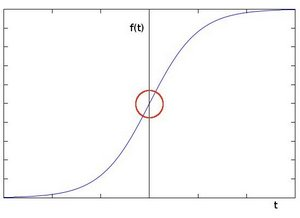
\includegraphics{graph1.jpg}
\caption{Graph - f(t)}
\end{figure}

However if we take the first derivative we can see the edge peak more
clearly as shown below:\\
\begin{figure}
	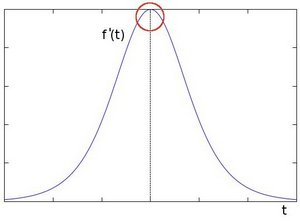
\includegraphics{graph2.jpg}
	\caption{Graph - f'(t)}
\end{figure}

Hence we can detect edges in an image by locating pixel locations where
the gradient is higher than its neighbors (or to generalize, higher than
a threshold).\\
We're going to look into two commonly used edge detection schemes - the
gradient (\textbf{Sobel} - first order derivatives) based edge detector
and the \textbf{Laplacian} (2nd order derivative, so it is extremely
sensitive to noise) based edge detector. Both of them work with
convolutions and achieve the same end goal - \emph{Edge Detection}.

\subsection{Sobel Edge Detection}\label{sobel-edge-detection}

The Sobel operator, sometimes called Sobel Filter is a discrete
differentiation operator, computing an approximation of the gradient of
the image intensity function.\\
Sobel edge detector is a gradient based method based on the first order
derivatives. It calculates the first derivatives of the image separately
for the X and Y axes.\\
The operator uses two 3X3 kernels which are convolved with the original
image to calculate approximations of the derivatives - one for
horizontal changes, and one for vertical. The picture below shows Sobel
Kernels in x-dir and y-dir:\\
\begin{figure}
\centering
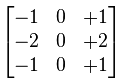
\includegraphics{sobelkernelx.png}
\caption{Sobel\_Kernel\_x}
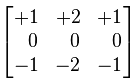
\includegraphics{sobelkernely.png}
\caption{Sobel\_Kernel\_y}
\end{figure}

\subsection{Scharr}\label{scharr}

\subsubsection{Working Principle}\label{working-principle}

Scharr operator is used to find image gradients(or edge detection). This
operator uses two kernels to convolve the image and calculate
derivatives in two directions. The derivatives track changes in
horizontal as well as vertical directions. Scharr operator tries to
overcome Sobel operator's drawback of not having perfect rotational
symmetry. The commonly used filter kernels are -

\begin{figure}[htbp]
\centering
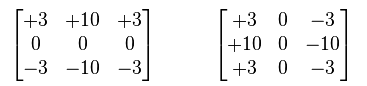
\includegraphics{Scharr_kernel.png}
\caption{Scharr kernel}
\end{figure}

The main function used for Scharr operator is-

\begin{Shaded}
\begin{Highlighting}[]
    \NormalTok{cv2.Scharr(src, ddepth, dx, dy[, dst[, scale[, delta[, borderType]]]])}
\end{Highlighting}
\end{Shaded}

where * \textbf{src} : Input image * \textbf{ddepth} : Output image
depth. Following are the compatible depths- \\
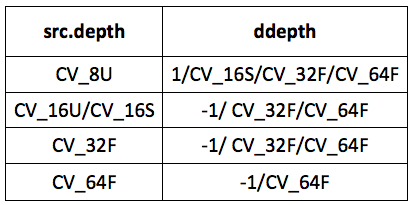
\includegraphics{table.png}

\begin{itemize}
\tightlist
\item
  \textbf{dst} : Output image of the same size and same number of
  channels as src.
\item
  \textbf{scale} : Optional scale factor for computed derivative values.
  No scaling is applied by default.
\item
  \textbf{delta} : Optional delta value that is added to results prior
  to storing them in dst.
\item
  \textbf{borderType}: Pixel extrapolation method
\end{itemize}

\subsubsection{Example}\label{example}

Consider the following image-

\begin{figure}[htbp]
\centering
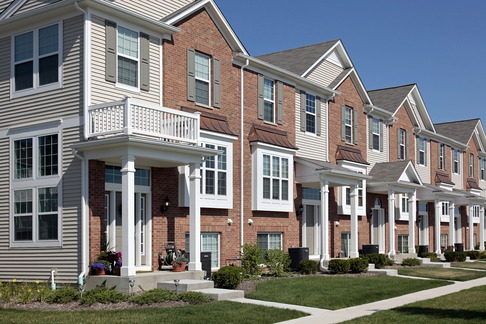
\includegraphics{house.jpg}
\caption{Example house}
\end{figure}

On applying Scharr operator on above image, we get the following-

\begin{figure}[htbp]
\centering
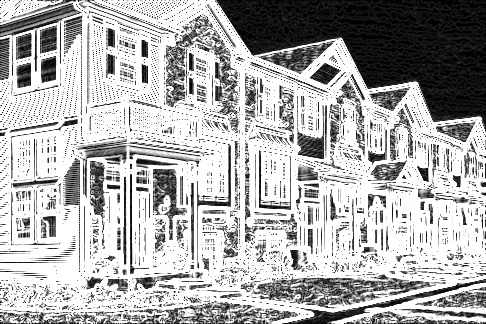
\includegraphics{Scharr.jpg}
\caption{Scharr image}
\end{figure}

\subsection{Laplacian Edge Detection}\label{laplacian-edge-detection}

The Laplacian edge detector uses only one kernel. It calculates second
order derivatives in a single pass. The Laplacian function is given
below:\\
\begin{figure}
\centering
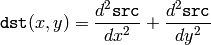
\includegraphics{laplace_func.png}
\caption{Laplace Function}
\end{figure}

A kernel used in this Laplacian detection looks like this:\\
\begin{figure}
\centering
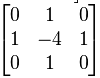
\includegraphics{LaplacianKernel.png}
\caption{laplacian Kernel}
\end{figure}
\subsection{Applications}\label{applications}

\begin{itemize}
\tightlist
\item
  These operators can be used to extract features from an image.
\item
  They used for edge detection, which is the basis for most image
  processing applications.
\end{itemize}

\section{Code}\label{code}

\subsection{Sobel and Laplacian}\label{sobel-and-laplacian}

\begin{verbatim}
#Import modules
import cv2
import numpy as np
import matplotlib.pyplot as plt

#Defining variables
scale = 1
delta = 0
ddepth = cv2.CV_64F

#Read the image
img = cv2.imread('lamp.jpg')

'''
OpenCV represents RGB images as multi-dimensional NumPy arrays…but in reverse
order!This means that images are actually represented in BGR order rather than
RGB!
'''
#Convert to RGB
img = cv2.cvtColor(img, cv2.COLOR_BGR2RGB)    

#Convert to grayscale
gray = cv2.cvtColor(img,cv2.COLOR_BGR2GRAY) 

#Applying threshold
ret, thresh = cv2.threshold(gray,127,255, cv2.THRESH_BINARY) 

# Gradient-X
grad_x = cv2.Sobel(thresh,ddepth,1,0,ksize = 3, scale = scale, 
delta = delta,borderType = cv2.BORDER_DEFAULT)

# Gradient-Y
grad_y = cv2.Sobel(thresh,ddepth,0,1,ksize = 3, scale = scale, 
delta = delta, borderType = cv2.BORDER_DEFAULT)

#Laplacian
lap = cv2.Laplacian(thresh,ddepth) 

# converting back to uint8
abs_grad_x = cv2.convertScaleAbs(grad_x)   
abs_grad_y = cv2.convertScaleAbs(grad_y)

#Finding the weighted mean
Sobel = cv2.addWeighted(grad_x,0.5,grad_y,0.5,0)

#Plotting the images
plt.subplot(3,2,1),plt.imshow(img,cmap = 'gray')
plt.title('Original'), plt.xticks([]), plt.yticks([])
plt.subplot(3,2,2),plt.imshow(grad_x,cmap = 'gray')
plt.title('Sobel x'), plt.xticks([]), plt.yticks([])
plt.subplot(3,2,3),plt.imshow(grad_y,cmap = 'gray')
plt.title('Sobel y'), plt.xticks([]), plt.yticks([])
plt.subplot(3,2,4),plt.imshow(Sobel,cmap = 'gray')
plt.title('Sobel'), plt.xticks([]), plt.yticks([])
plt.subplot(3,2,5),plt.imshow(lap,cmap = 'gray')
plt.title('Laplacian'), plt.xticks([]), plt.yticks([])

#Display the window
plt.show()
\end{verbatim}

\begin{figure}[htbp]
\centering
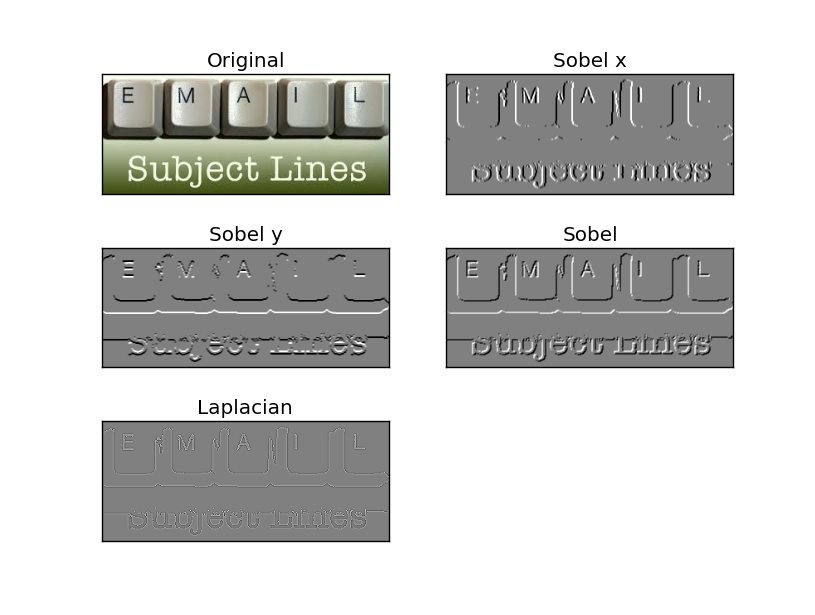
\includegraphics{Sobel1.png}
\caption{Output Image}
\end{figure}

\subsection{Scharr}\label{scharr-1}

\begin{itemize}
\item
  Let us first import opencv package and read our image.

\begin{Shaded}
\begin{Highlighting}[]
\ImportTok{import} \NormalTok{cv2}
\NormalTok{img }\OperatorTok{=} \NormalTok{cv2.imread(‘example.jpg’)}
\end{Highlighting}
\end{Shaded}
\item
  Now, we remove noise from image using Gaussian Blur and then convert
  it to grayscale.

\begin{Shaded}
\begin{Highlighting}[]
\NormalTok{img }\OperatorTok{=} \NormalTok{cv2.GaussianBlur(img, (}\DecValTok{3}\NormalTok{,}\DecValTok{3}\NormalTok{), }\DecValTok{0}\NormalTok{)}
\NormalTok{gray }\OperatorTok{=} \NormalTok{cv2.cvtColor(img, cv2.COLOR_BGR2GRAY)}
\end{Highlighting}
\end{Shaded}
\item
  The next step is to find gradients in x- and y directions.

\begin{Shaded}
\begin{Highlighting}[]
\NormalTok{grad_x }\OperatorTok{=} \NormalTok{cv2.Scharr(gray, cv2.CV_16S, }\DecValTok{1}\NormalTok{, }\DecValTok{0}\NormalTok{) }\CommentTok{#Gradient X}
\NormalTok{grad_y }\OperatorTok{=} \NormalTok{cv2.Scharr(gray, cv2.CV_16S, }\DecValTok{0}\NormalTok{, }\DecValTok{1}\NormalTok{) }\CommentTok{#Gradient Y}
\end{Highlighting}
\end{Shaded}
\item
  The gradients should now be converted back to unsigned 8-bit integer
  form.

\begin{Shaded}
\begin{Highlighting}[]
\NormalTok{abs_grad_x }\OperatorTok{=} \NormalTok{cv2.convertScaleAbs(grad_x)}
\NormalTok{abs_grad_y }\OperatorTok{=} \NormalTok{cv2.convertScaleAbs(grad_y)}
\end{Highlighting}
\end{Shaded}
\item
  We can now obtain our Scharr derivative by adding these two gradients.

\begin{Shaded}
\begin{Highlighting}[]
\NormalTok{scharr }\OperatorTok{=} \NormalTok{cv2.add(abs_grad_x, abs_grad_y)}
\end{Highlighting}
\end{Shaded}
\item
  Finally, we display our result.

\begin{Shaded}
\begin{Highlighting}[]
\NormalTok{cv2.imshow(‘Scharr Derivative’, scharr)}
\NormalTok{cv2.waitKey(}\DecValTok{0}\NormalTok{)}
\NormalTok{cv2.destroyAllWindows()}
\end{Highlighting}
\end{Shaded}
\end{itemize}

\section{References}\label{references}

\begin{enumerate}
\def\labelenumi{\arabic{enumi}.}
\item \href{https://github.com/eyantrainternship/eYSIP_2015_Marker_based_Robot_Localisation/blob/master/Task-3/Gradients/src/gradients.py}{Code - Github link}

\item
  \href{http://opencv-python-tutroals.readthedocs.org/en/latest/py\_tutorials/py\_imgproc
  /py\_gradients/py\_gradients.html}{Gradients - opencv and python tutorials}
\item
  \href{http://www.bogotobogo.com/python/OpenCV\_Python/python\_opencv3\_Image\_Gradient
  \_Sobel\_Laplacian\_Derivatives\_Edge\_Detection.php}{Gradients - More info}
\item
  \href{http://en.wikipedia.org/wiki/Sobel\_operator}{Sobel Operator}
\item
  \href{http://docs.opencv.org/doc/tutorials/imgproc/imgtrans/sobel
  \_derivatives/sobel\_derivatives.html}{OpenCv docs}
\end{enumerate}

\section{Excercises}\label{excercises}

\end{document}
